% GAD block split of the NTK feature map matrix M, with the CK as the modeled block.
% Standalone: compile with pdflatex. To use in the paper, copy the tikzpicture and add
% \usetikzlibrary{decorations.pathreplacing,calc} to the preamble.
\documentclass[tikz,border=4pt]{standalone}
\usepackage{amsmath,amssymb}
\usetikzlibrary{decorations.pathreplacing,calc}

\begin{document}
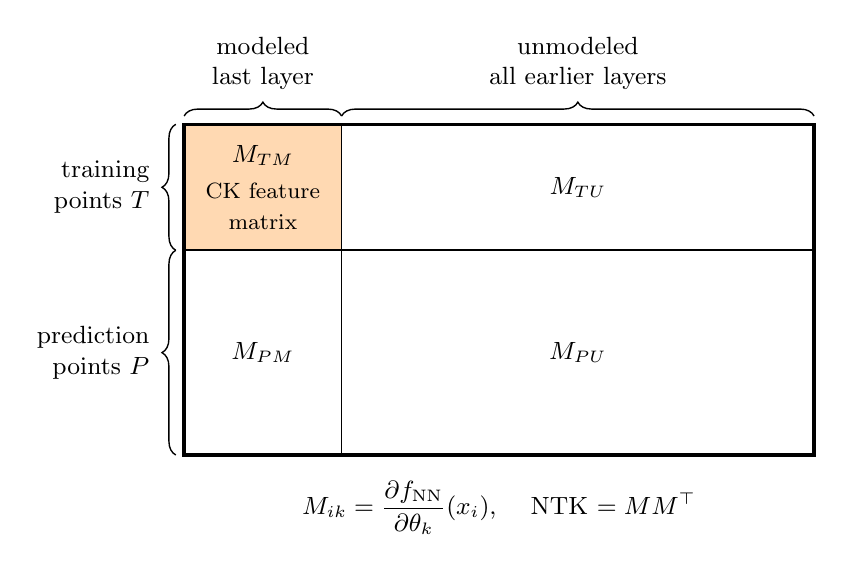
\begin{tikzpicture}[
    font=\small,
    block/.style={draw=black, line width=0.6pt},
    brace/.style={decorate, decoration={brace, amplitude=5pt, raise=3pt}, line width=0.5pt},
  ]
  % ---- geometry: modeled (CK) columns narrow, unmodeled wide; few training rows, more test rows
  \def\wM{2.0}   % width of the modeled (last-layer) columns
  \def\wU{6.0}   % width of the unmodeled columns
  \def\hT{1.6}   % height of the training-point rows
  \def\hP{2.6}   % height of the prediction-point rows

  % ---- the four blocks (y grows upward, so T sits on top)
  \fill[orange!30] (0,\hP) rectangle (\wM,\hP+\hT);
  \draw[block] (0,\hP)   rectangle (\wM,\hP+\hT)      node[pos=.5, align=center] {$M_{TM}$\\[2pt] \footnotesize CK feature\\ \footnotesize matrix};
  \draw[block] (\wM,\hP) rectangle (\wM+\wU,\hP+\hT)  node[pos=.5] {$M_{TU}$};
  \draw[block] (0,0)     rectangle (\wM,\hP)          node[pos=.5] {$M_{PM}$};
  \draw[block] (\wM,0)   rectangle (\wM+\wU,\hP)      node[pos=.5] {$M_{PU}$};
  \draw[line width=1.2pt] (0,0) rectangle (\wM+\wU,\hP+\hT);

  % ---- column braces (top)
  \draw[brace] (0,\hP+\hT) -- (\wM,\hP+\hT)
    node[midway, above=9pt, align=center] {modeled\\ last layer};
  \draw[brace] (\wM,\hP+\hT) -- (\wM+\wU,\hP+\hT)
    node[midway, above=9pt, align=center] {unmodeled\\ all earlier layers};

  % ---- row braces (left)
  \draw[brace] (0,\hP) -- (0,\hP+\hT)
    node[midway, left=9pt, align=right] {training\\ points $T$};
  \draw[brace] (0,0) -- (0,\hP)
    node[midway, left=9pt, align=right] {prediction\\ points $P$};

  % ---- what M is
  \node[below=6pt, align=center] at ($(0.5*\wM+0.5*\wU,0)$)
    {$M_{ik} = \dfrac{\partial f_{\mathrm{NN}}}{\partial \theta_k}(x_i)$, \quad
     NTK $= M M^{\top}$};
\end{tikzpicture}
\end{document}
